
%\documentclass[manuscript]{acmart}
%\documentclass[acmsmall]{acmart}
%\settopmatter{printacmref=false}


\documentclass[
  a4paper,
  12pt,
  DIV=12,        % höherer Wert = schmalere Ränder, weniger Whitespacmi
  parskip=half,  % Absätze mit halbem Abstand statt Einzug
  headings=small % kleinere Überschriften, weniger vertikaler Abstand
]{scrartcl}

%\documentclass[a4paper,11pt]{scrartcl}
%\documentclass[a4paper,11pt]{report}
%\documentclass[a4paper,12pt]{book}
\usepackage[utf8]{inputenc}
\usepackage[german]{babel}
\usepackage[T1]{fontenc}
\usepackage{lmodern}
\usepackage[inkscapelatex=false]{svg}
% Texte im SVG von Inkscape setzen lassen, nicht durch die Dokumentschrift ersetzen
\svgsetup{inkscapelatex=false}
\usepackage{amsmath}
\usepackage{caption}
\usepackage{gensymb}
\usepackage{microtype}
\usepackage{longtable}
\usepackage{tabularx}   % Spalten, die die restliche Zeilenbreite auffüllen (X-Spalte)
\usepackage{booktabs}   % \toprule \midrule \bottomrule (in mobrob_table.tex verwendet)
\usepackage{wrapfig}    % Textumfluss um Abbildungen

\usepackage[citecolor=black, colorlinks=true, linkcolor=black, urlcolor=blue]{hyperref}


%\usepackage{geometry}
\usepackage{siunitx}
%\geometry{margin=2.5cm}


\usepackage{amsthm}
\usepackage{mdframed}
\usepackage{enumitem}

\newmdtheoremenv{theorem}{Theorem}

\theoremstyle{definition}
\newmdtheoremenv{derivation}{Derivation}


%\mdfdefinestyle{leftline}{
%    topline=false, bottomline=false, rightline=false,
%    linewidth=2pt, linecolor=gray
%}
\theoremstyle{definition}
\newmdtheoremenv[style=leftline]{myalgorithm}{Algorithm}




%\usepackage{fancyvrb}







\let\Bbbk\relax
\usepackage{amssymb}


\usepackage{yfonts}

\usepackage{kvmap}

\usepackage[
    backend=biber,
    style=alphabetic,
    sortlocale=de_DE,
    natbib=true,
    %url=false,
    doi=true,
    %eprint=false
]{biblatex}
\addbibresource{Literaturrecherche-Stefan-Etringer/algo-references.bib}

\usepackage[
    backend=biber,
    style=alphabetic,
    sortlocale=de_DE,
    natbib=true,
    %url=false,
    doi=true,
    %eprint=false
]{biblatex}
\addbibresource{Literaturrecherche-Dennis/mobrob_references.bib}

\usepackage[autostyle=true,german=quotes]{csquotes}
\usepackage{trfsigns} %fourier transform arrow
\usepackage{mathrsfs} %fourier F
\usepackage{commath}

\usepackage{pgfplots}
\pgfplotsset{compat=1.18}

\usepackage{xcolor}
\usepackage{listings}
\usepackage[european]{circuitikz}
\ctikzset{tripoles/european not symbol=ieee circle}

%\usepackage[shading]{moeptikz}
%\moeptikzset{shading=true}

%\usepackage{german,longtable}

\usepackage{xcolor}
\usepackage{color}
\usepackage{url}

\usepackage{xfrac}

\usepackage{listings}
\usepackage{verbatimbox}

\usepackage{algorithm}
\usepackage{algpseudocode}

\usepackage{multirow}
\usepackage{float}
\usepackage{pdflscape}   % einzelne Querformatseiten (im PDF gedreht)

%%%% TIKZ

\usepackage{tikz}

\usepackage{pgfplots}
\usetikzlibrary{calc,
trees,positioning,arrows,
chains,shapes.geometric,
decorations.pathreplacing,
decorations.pathmorphing,shapes,
matrix,shapes.symbols,
plotmarks}
%\tikzexternalize[prefix=figures/]

%\tikzset{%
%  block/.style    = {draw, thick, rectangle, minimum height = 3em,
%    minimum width = 3em},
%  sum/.style      = {draw, circle, node distance = 2cm}, % Adder
%  input/.style    = {coordinate}, % Input
%  output/.style   = {coordinate} % Output
%}
% Defining string as labels of certain blocks.
%\newcommand{\suma}{\Large$+$}
%\newcommand{\multa}{\Large$\times$}
%\newcommand{\inte}{$\displaystyle \int$}
%\newcommand{\derv}{\huge$\frac{d}{dt}$}

\usetikzlibrary{arrows,automata,positioning}
%\usepackage{automata}


%%% END TIKZ

\usepackage[section]{placeins}

\usepackage{textcomp}


\usepackage{listings}
\usepackage{verbatimbox}

\usepackage{bold-extra}

\usepackage{framed}

%\usepackage{fancyhdr}
%\pagestyle{fancy}
%\lhead{\leftmark}
%\chead{}
%\rhead{}
%\lfoot{}
%\cfoot{\thepage}
%\rfoot{}
%\renewcommand{\headrulewidth}{0.2pt}
%\renewcommand{\footrulewidth}{0.2pt}



\newcommand{\Z}{\mathbb{Z}}
\newcommand{\R}{\mathbb{R}}
\newcommand{\C}{\mathbb{C}}
\newcommand{\N}{\mathbb{N}}
\newcommand{\SqrtNy}{$\sqrt{\textsc{Ny}}$}
\newcommand{\conj}{\overline}
\newcommand{\Kset}{\textswab{K}}
\newcommand{\Qset}{\textswab{Q}}
\newcommand{\ceil}[1]{\left\lceil #1 \right\rceil}
\newcommand{\floor}[1]{\left\lfloor #1 \right\rfloor}
\newcommand{\sorted}[1]{\textsc{sort}\left\lbrace #1 \right\rbrace}
\newcommand{\SNRgain}{a_{SNR}}
\newcommand{\EQgain}{a_{EQ}}
\newcommand{\SIRgain}{a_{SIR}}
\newcommand{\SNIRgain}{a_{SINR}}
\newcommand{\SNR}{\textsc{SNR}}
\newcommand{\CIRgain}{a_{CIR}}
\newcommand{\CINRgain}{a_{CINR}}
\newcommand{\CNR}{\textsc{CNR}}
\newcommand{\CINR}{\textsc{CINR}}
\newcommand{\HPAModel}{ Hughes 1177H TWTA }
\newcommand{\bigO}{\mathcal{O}}
\newcommand{\CopWinCompl}{2.375377}
\newcommand{\IBO}{\textsc{IBO}}
\newcommand{\OBO}{\textsc{OBO}}
\newcommand{\spacepage}{\newpage\null\thispagestyle{empty}\newpage}
\newcommand{\satcom}{ SatCom }
\newcommand{\db}{~\text{dB}}


\definecolor{mGreen}{rgb}{0,0.6,0}
\definecolor{mGray}{rgb}{0.5,0.5,0.5}
\definecolor{mPurple}{rgb}{0.58,0,0.82}
\definecolor{backgroundColour}{rgb}{0.95,0.95,0.92}

\lstdefinestyle{CStyle}{
    backgroundcolor=\color{backgroundColour},
    commentstyle=\color{mGreen},
    keywordstyle=\color{magenta},
    numberstyle=\tiny\color{mGray},
    stringstyle=\color{mPurple},
    basicstyle=\footnotesize,
    breakatwhitespace=false,
    breaklines=true,
    captionpos=b,
    keepspaces=true,
    numbers=left,
    numbersep=5pt,
    showspaces=false,
    showstringspaces=false,
    showtabs=false,
    tabsize=2,
    language=C
}

\lstdefinelanguage{VHDL}{
  morekeywords=[1]{library,use,all,entity,is,port,in,out,end,architecture,of,begin,process,if,then,else,elsif,when,others,signal,variable,wait,for,loop},
  morecomment=[l]--,
  morestring=[b]",
  sensitive=true
}

\lstset{
  language=VHDL,
  basicstyle=\ttfamily\small,
  keywordstyle=\color{blue},
  commentstyle=\color{gray},
  stringstyle=\color{red},
  numbers=left,
  numberstyle=\tiny,
  stepnumber=1,
  numbersep=8pt,
  frame=single,
  breaklines=true,
  captionpos=b
}

\lstset{numbers=none}

%\newcounter{example}
%\renewcommand{\theexample}{\thesection.\arabic{example}}


% Default fixed font does not support bold face
\DeclareFixedFont{\ttb}{T1}{txtt}{bx}{n}{12} % for bold
\DeclareFixedFont{\ttm}{T1}{txtt}{m}{n}{12}  % for normal

% Custom colors
\usepackage{color}
\definecolor{deepblue}{rgb}{0,0,0.5}
\definecolor{deepred}{rgb}{0.6,0,0}
\definecolor{deepgreen}{rgb}{0,0.5,0}

\usepackage{listings}

% Python style for highlighting
\newcommand\pythonstyle{\lstset{
language=Python,
basicstyle=\ttm,
morekeywords={self},              % Add keywords here
keywordstyle=\ttb\color{deepblue},
emph={MyClass,__init__},          % Custom highlighting
emphstyle=\ttb\color{deepred},    % Custom highlighting style
stringstyle=\color{deepgreen},
frame=tb,                         % Any extra options here
showstringspaces=false
}}


% Python environment
\lstnewenvironment{python}[1][]
{
\pythonstyle
\lstset{#1}
}
{}

% Python for external files
\newcommand\pythonexternal[2][]{{
\pythonstyle
\lstinputlisting[#1]{#2}}}

% Python for inline
\newcommand\pythoninline[1]{{\pythonstyle\lstinline!#1!}}





\nocite{*}


\begin{document}
%\pagenumbering{roman}



\title{Coasterbot}
\subtitle{Phasenpaper M0}
\author{Gereon Such}
%\email{gereonsuch@suchdsp.com}
%\affiliation{
%  \institution{Wilhelm Büchner University of Applied Sciences}
%  \department{Computer Engineering}
%  \city{Hof}
%  \country{Germany}
%}



\begin{titlepage}
  \begin{center}
    {\large Wilhelm Büchner University of Applied Sciences} \\[0.3em]

    {\normalsize Projektseminar Master}
\vspace{5em}

    {\LARGE\bfseries Coasterbot} \\[0.5em]

    {\large Phasenpaper M0} \\[1em]

    {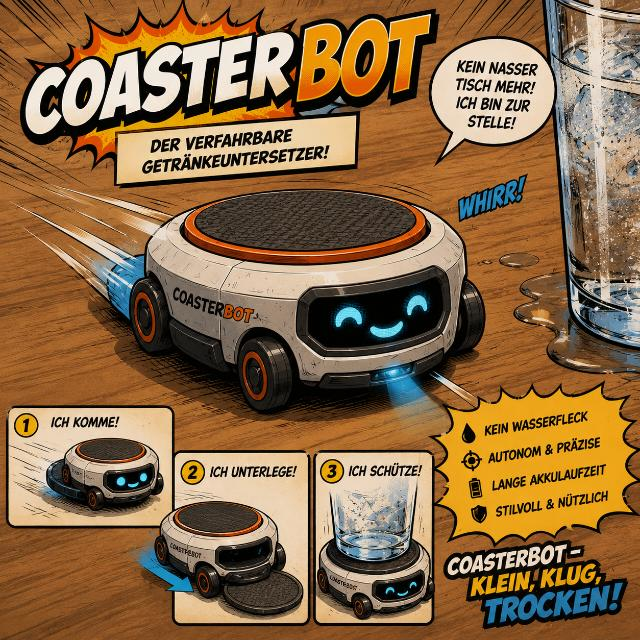
\includegraphics[width=0.38\textwidth]{coasterbot.png}} \\[1em]

\vspace{4em}

    {\normalsize
\begin{tabular}{ll}
Dennis Borutta, B. Eng & dennis.borutta@outlook.com\\
Stefan Etringer, B. Eng & mail@stefan.works\\
Gereon Such, M. Sc. & gereonsuch@gmail.com\\
\end{tabular}
    }
  \end{center}


\end{titlepage}


% einleitung preambel etc.


% Versionshistorie des Dokuments -- eigene Seite direkt nach dem Titelblatt
\section*{Versionshistorie}

\begin{tabularx}{\textwidth}{@{}clp{2.6cm}X@{}}
\toprule
\textbf{Version} & \textbf{Datum} & \textbf{Bearbeiter} & \textbf{Änderungen}\\
\midrule
1 & 20.07.2026 & Such & Erstfassung des Phasenpapiers M0\\
2 & 21.07.2026 & Etringer & Literaturrecherche zu Algorithmen ergänzt\\
3 & 21.07.2026 & Borutta, Such & Literaturrecherche und Einleitungstext ergänzt; Coasterbot-Abbildung eingefügt; Timeline und Projektzeitraum angepasst\\
4 & 22.07.2026 & Such & Versionshistorie ergänzt\\
5 & 23.07.2026 & Borutta & Projektsteckbrief in Tabelle umgewandelt. Dokumentenstruktur angepasst.\\
6 & 24.07.2026 & Etringer & Links und Referenzen klickbar,
  Rechtschreibfehler, Change: - to emdash bei einem Satz, hyperlink zu unserem
  Notion and git repo hinzugefügt, fehlende Kurzreferenz für Handbook of
  Robotics hinzugefügt, Leerzeichen aus in gctronic.com URL entfernt,
  Encodingfehler mit den tiefen Anführungszeichen vor Introduction to
  Algorithms Namen gelöst, Linting \\
7 & 25.07.2026 & Such & Graphen aktualisiert \\
8 & 25.07.2026 & Such, Borutta, Etringer & Überschrift Anhang, anpassen der Tabelle im Anhang\\
9 & 25.07.2026 & Such & Vorgangstabelle eingefügt\\
10 & 30.07.2026 & Etringer & Erweiterung der Out-of-Scope Tabelle nach Absprache in M0, Literaturrecherche als Kapitel und im Anhang hinzugefügt\\
\bottomrule
\end{tabularx}


\newpage

\tableofcontents

\newpage


\section{Projektübersicht}

\begin{longtable}{@{}p{0.3\textwidth}p{0.7\textwidth}@{}}
\toprule
\textbf{Kategorie} & \textbf{Inhalt} \\
\midrule
\endfirsthead
\toprule
\textbf{Kategorie} & \textbf{Inhalt} \\
\midrule
\endhead

Projektname & Coasterbot -- Entwicklung eines Prototyps \\
\midrule

Projektzeitraum & Beginn: \textbf{15.07.2026} \quad | \quad Abschluss: \textbf{07.11.2026}\\
\midrule

Projektziel & Entwicklung eines Prototyps eines Coasterbots: ein handtellergro{\ss}er Roboter, der selbstst\"andig auf einem Tisch navigiert, dort Getr\"ankeuntersetzer in Richtung von Personen ausgibt und diese automatisiert wieder aufnimmt. \\
\midrule

Weitere Ausbaustufen (Nicht im Fokus) & Automatisierte Tischreinigung, Aufnahme von Bestellungen, Initialisierung von Bezahlvorg\"angen \\
\midrule



Motivation / Nutzen &
\vspace{-\baselineskip}
\begin{itemize}[partopsep=0pt, topsep=6pt, itemsep=2pt]
  \item Entlastung des Bedienpersonals durch reduzierten Aufgabenbereich unterstützt damit den de seit Jahren bestehenden Fachkräftemangels in der Gastronomie~\cite{DEHOGA2025Q4}
  \item Alleinstellungsmerkmal und zusätzliches Attraktivitätsmerkmal f\"ur Bars/Restaurants
  \item Potenziell mehr positive Bewertungen und verbesserte Online-Pr\"asenz und damit Positiver Einfluss auf den Umsatz (Online-Pr\"asenz als zunehmend relevanter Faktor bei der Restaurantwahl)~\cite{BibEntry2026Jul}
\end{itemize} \\
\midrule


Definition of Done &
\vspace{-\baselineskip}
\begin{itemize}[partopsep=0pt, topsep=6pt, itemsep=2pt]
  \item STL-Dateien und Schaltpl\"ane zur Fertigung eines Prototypen sind fertiggestellt
  \item Softwarearchitektur und -komponenten sind ausgearbeitet
  \item Eine Simulation des Programmablaufes ist erstellt und validiert
  \item Tests, die sich aus den Anforderungen ergeben, sind identifiziert und definiert
\end{itemize} \\
\midrule

Out of Scope &
\vspace{-\baselineskip}
\begin{itemize}[partopsep=0pt, topsep=6pt, itemsep=2pt]
  \item EMV-Betrachtungen
  \item Kartierung oder dauerhafte Modellierung der Umgebung
  \item Einbindung in ein Netzwerk oder Cloud-Dienste
  \item Marketing- und Wirtschaftlichkeitskonzepte
  \item Schwarmverhalten mehrerer Coasterbots
  \item Automatisierte Tischreinigung
  \item Automatisierter Austausch der Coaster
  \item Getränketransport als Primärfunktion des Systems
  \item Betrieb mit aufladbarem Akkumulator
\end{itemize} \\
\bottomrule

\end{longtable}

\section{Projektorganisation}

Das Projektteam besteht aus den drei Mitgliedern

\begin{center}
\begin{tabular}{lll}
Dennis Burutta & Leiter/Mitglied & dennis.borutta@outlook.com\\
Stefan Etringer & Admin/Mitglied & mail@stefan.works \\
Gereon Such & Mitglied & gereonsuch@gmail.com\\
\end{tabular}
\end{center}




Für die Projektorganisation und dokumentenbasierte Kommunikation im Team wird
das Tool Notion \url{https://app.notion.com} genutzt. In diesem werden
\href{https://app.notion.com/p/Projektarbeit-39a745ea234f80d4b39ace9b616a41de}{Projektphasen,Arbeitspakete, Fortschritt, Ergebnisse sowie Meilensteine}
protokolliert.
Notion bietet hier vielfältige Planungsmöglichkeiten sowie Visualisierungen
dazu. Eine Besonderheit dabei ist, dass Notion die Möglichkeit bietet
kollaborativ an Dokumenten zu arbeiten und diese direkt an Arbeitspaketen zu
knüpfen. So können die Arbeitsergbnisse und Referenzen strukturiert abgelegt
werden.

Entwicklungsrelevante Dateien wie Source Code, CAD-Dateien für das Chassis oder Schaltungen werden in einem \href{https://github.com/Project-CoasterBot/coasterbot}{gemeinsamen Git Repository} abgelegt. % ich lasse hier einfach offen wo und wie, ob github oder gitlab oder whatever...

Zur Remote Kommunikation wird eine Kombination aus Instant Messaging für kurzfristige Information und Absprachen sowie regelmäßigen Videocalls mit dem Tool Alfaview \url{https://alfaview.com} genutzt.




\section{Projektplanung}

Mit Hilfe der Tools Draw.io und Notion wird im Team die Projektplanung durchgeführt. Hierzu wird zur Ermittlung notwendiger Teilaufgaben und Arbeitspakete die Kreativmethode der Mind-Map angewandt. Daraus ergibt sich der Projektstrukturplan mit Arbeitspaketen. Aus diesem wird anschließend eine Vorgangsliste in ProjectLibre erstellt, die in einem Netzplan überführt wird. Mit Hilfe des Netzplanes wird anschließend ein detaillierter Zeitplan in Notion erstellt.

\subsection{Projektstruktur}
Zur weiteren Bestimmung von erforderlichen Teilaufgaben und Arbeitspaketen wurde die Kreativmethode der Mind-Map angewandt. Die Ergebnisse hierzu sind in Abbildung~\ref{arbeitspaketemindmap} zu sehen. Daraus ergibt sich der Projektstrukturplan mit Arbeitspaketen wie in Abbildung~\ref{projektstrukturplan} gezeigt. Hierbei wird ersichtlich, dass der Strang ``Organisation''   aus der Mind-Map nicht in dem Projektstrukturplan zu sehen ist. Dies wird begründet, da es sich dabei um fortlaufende Aufgaben handelt, die über die gesamte Projektlaufzeit hinweggeführt werden.

\begin{figure}[htbp]
  \centering
  \includesvg[scale=0.4]{MindMap.svg}
  \caption{Mindmap zur Projektstruktur}\label{arbeitspaketemindmap}
\end{figure}

\begin{figure}[htbp]
  \centering
  \includesvg[scale=0.45]{Projektstrukturplan.svg}
  \caption{Projektstrukturplan}\label{projektstrukturplan}
\end{figure}

\newpage
\subsection{Netzplan}
Mit dem Zeithorizont von 4 Monaten ergibt sich mit Gewichtung der jeweiligen Arbeitspakete nach Aufwand und Priorität der in Abbildung~\ref{fig:netzplan} dargestellte Netzplan nach DIN 69900. Aufgrund seiner Breite ist dieser auf einer eigenen Seite im Querformat abgebildet. Folgende Tabelle aus ProjectLibre wurde als Grundlage für den Graphen genutzt, die Graphik selbst per LLM aus der Tabelle erstellt.




\begin{tabularx}{\textwidth}{cX@{}ccccccc}
\toprule
\footnotesize
\textbf{ID} & \footnotesize\textbf{Arbeitspaket} & \footnotesize\textbf{Dauer} & \footnotesize\textbf{FAZ} & \footnotesize\textbf{FEZ} & \footnotesize\textbf{SAZ} & \footnotesize\textbf{SEZ} & \footnotesize\textbf{Kritisch}\\
\midrule
\footnotesize 1001 & \footnotesize Steckbrief\-definition &	\footnotesize 1 &	\footnotesize 15.07.26 & \footnotesize 15.07.26	 & \footnotesize 09.10.26	 & \footnotesize 09.10.26 & 	 \footnotesize 	nein \\
\footnotesize 1002	 & \footnotesize Projekt\-organisation und Planung & 	\footnotesize 4	 & \footnotesize 16.07.26	 & \footnotesize 19.07.26	 & \footnotesize 10.10.26	 & \footnotesize 13.10.26	& \footnotesize nein \\
\footnotesize 1010	 & \footnotesize Algorithmik recherchieren & 	\footnotesize 8	 & \footnotesize 15.07.26	 & \footnotesize 22.07.26	 & \footnotesize 15.07.26	 & \footnotesize 22.07.26	 & 	\footnotesize ja \\
\footnotesize 1020 & \footnotesize Marktsichtung durchführen & \footnotesize 	8	 & \footnotesize 15.07.26	 & \footnotesize 22.07.26 & \footnotesize 	15.07.26 & \footnotesize 	22.07.26 &  \footnotesize ja \\
\footnotesize 1030	 & \footnotesize Stand zu Mobile Robotik recherchieren	 & \footnotesize 8	 & \footnotesize 15.07.26	 & \footnotesize 22.07.26	 & \footnotesize 15.07.26	 & \footnotesize 22.07.26	 & \footnotesize ja\\
\footnotesize 101	 & \footnotesize Dokumente zusammentragen	 & \footnotesize 3	 & \footnotesize 23.07.26 & \footnotesize 	25.07.26	 & \footnotesize 14.10.26 & \footnotesize 	16.10.26	 & \footnotesize nein \\
\footnotesize 2010	 & \footnotesize Anwendungsfälle definieren	 & \footnotesize 3	 & \footnotesize 23.07.26	 & \footnotesize 25.07.26 & \footnotesize 	23.07.26	 & \footnotesize 25.07.26	 & \footnotesize 	ja \\
\footnotesize 2020 & \footnotesize 	Maturity Level definieren	 & \footnotesize 4 & \footnotesize 	26.07.26 & \footnotesize 	29.07.26	 & \footnotesize 26.07.26	 & \footnotesize 29.07.26	  & \footnotesize ja \\
\footnotesize 2030 & \footnotesize 	Lastenheft erstellen	 & \footnotesize 7 & \footnotesize 	30.07.26 & \footnotesize 	05.08.26	 & \footnotesize 30.07.26	 & \footnotesize 05.08.26	  & \footnotesize ja\\
\footnotesize 3010 & \footnotesize 	Testfälle definieren	 & \footnotesize 5	 & \footnotesize 06.08.26	 & \footnotesize 10.08.26 & \footnotesize 10.08.26 & \footnotesize 14.08.26 & \footnotesize nein \\
\footnotesize 3020 & \footnotesize Sensorik/Aktorik auswählen & \footnotesize 5 & \footnotesize 06.08.26 & \footnotesize 10.08.26 & \footnotesize 06.08.26 & \footnotesize 10.08.26 & \footnotesize ja \\
\footnotesize 3030 & \footnotesize Softwarearchitektur erarbeiten & \footnotesize 5 & \footnotesize 06.08.26 & \footnotesize 10.08.26 & \footnotesize 10.08.26 & \footnotesize 14.08.26 & \footnotesize nein \\
\footnotesize 3040 & \footnotesize Kostenkalkulation durchführen & \footnotesize 4 & \footnotesize 11.08.26 & \footnotesize 14.08.26 & \footnotesize 11.08.26 & \footnotesize 14.08.26 & \footnotesize ja \\
\footnotesize 3050 & \footnotesize Pflichtenheft erstellen & \footnotesize 8 & \footnotesize 15.08.26 & \footnotesize 22.08.26 & \footnotesize 15.08.26 & \footnotesize 22.08.26 & \footnotesize ja \\
\footnotesize 201 & \footnotesize Dokumente zusammentragen & \footnotesize 2 & \footnotesize 23.08.26 & \footnotesize 24.08.26 & \footnotesize 15.10.26 & \footnotesize 16.10.26 &  \footnotesize nein \\
\footnotesize 4010 & \footnotesize Bauteile beschaffen & \footnotesize 14 & \footnotesize 23.08.26 & \footnotesize 05.09.26 & \footnotesize 24.08.26 & \footnotesize 06.09.26 & \footnotesize nein \\
\footnotesize 4020 & \footnotesize Softwaretest erstellen & \footnotesize 10 & \footnotesize 23.08.26 & \footnotesize 01.09.26 & \footnotesize 23.08.26 & \footnotesize 01.09.26 & \footnotesize ja \\
\footnotesize 4030 & \footnotesize Software implementieren & \footnotesize 15 & \footnotesize 02.09.26 & \footnotesize 16.09.26 & \footnotesize 02.09.26 & \footnotesize 16.09.26 & \footnotesize ja \\
\footnotesize 4040 & \footnotesize Prototyp aufbauen & \footnotesize 10 & \footnotesize 06.09.26 & \footnotesize 15.09.26 & \footnotesize 07.09.26 & \footnotesize 16.09.26 & \footnotesize nein \\
\footnotesize 5000 & \footnotesize Test durchführen & \footnotesize 8 & \footnotesize 17.09.26 & \footnotesize 24.09.26 & \footnotesize 17.09.26 & \footnotesize 24.09.26 & \footnotesize ja \\
\footnotesize 6000 & \footnotesize Maturity Level feststellen & \footnotesize 5 & \footnotesize 25.09.26 & \footnotesize 29.09.26 & \footnotesize 25.09.26 & \footnotesize 29.09.26 & \footnotesize ja \\
\footnotesize 301 & \footnotesize Dokumente zusammentragen & \footnotesize 3 & \footnotesize 30.09.26 & \footnotesize 02.10.26 & \footnotesize 30.09.26 & \footnotesize 02.10.26 & \footnotesize ja \\
\footnotesize 401 & \footnotesize Endbericht erstellen und abgeben & \footnotesize 6 & \footnotesize 03.10.26 & \footnotesize 08.10.26 & \footnotesize 03.10.26 & \footnotesize 08.10.26 & \footnotesize ja \\
\footnotesize 7000 & \footnotesize Präsentation ausarbeiten & \footnotesize 8 & \footnotesize 09.10.26 & \footnotesize 16.10.26 & \footnotesize 09.10.26 & \footnotesize 16.10.26 & \footnotesize ja \\

\bottomrule
\end{tabularx}















\begin{landscape}
\thispagestyle{empty}   % keine Seitenzahl, Plan darf bis an den Papierrand
\null\vfill
% Auf dem Papier zentrieren, nicht im Satzspiegel: in der gedrehten Achse liegt
% der Satzspiegel nicht mittig (vorn 1in+topmargin+headheight+headsep, hinten Rest).
% Ausgleich = halbe Differenz der beiden Raender; die 3.8pt gleichen den
% asymmetrischen Weissraum im SVG selbst aus (viewBox: links 70, rechts 40).
% (in der landscape-Umgebung ist \linewidth die Ausdehnung entlang dieser Achse)
\noindent\hspace*{\dimexpr1in + \topmargin + \headheight + \headsep
                  - (\paperheight-\linewidth)/2 - 3.8pt\relax}%
\makebox[\linewidth]{%
  \begin{minipage}{\dimexpr\paperheight-2.4cm\relax}
    \centering
    \includesvg[width=\linewidth]{Coasterbot_Netzplan_v4.svg}
    \captionof{figure}{Netzplan}
\label{fig:netzplan}
  \end{minipage}}
\vfill
\end{landscape}


\begin{landscape}
\subsection{Zeitplan}
Mit Hilfe des Netzplanes wird der Zeitplan detailliert. Dieser ist in Abbildung \ref{fig:notiontimeline_full} reduziert abgebildet.

%\thispagestyle{empty}   % keine Seitenzahl, Plan darf bis an den Papierrand
%\null\vfill


% Auf dem Papier zentrieren, nicht im Satzspiegel: in der gedrehten Achse liegt
% der Satzspiegel nicht mittig (vorn 1in+topmargin+headheight+headsep, hinten Rest).
% Ausgleich = halbe Differenz der beiden Raender; die 3.8pt gleichen den
% asymmetrischen Weissraum im SVG selbst aus (viewBox: links 70, rechts 40).
% (in der landscape-Umgebung ist \linewidth die Ausdehnung entlang dieser Achse)
\noindent\hspace*{\dimexpr1in + \topmargin + \headheight + \headsep
                  - (\paperheight-\linewidth)/2 - 3.8pt\relax}%
\makebox[\linewidth]{%
  \begin{minipage}{\dimexpr\paperheight-2.4cm\relax}
    \centering
    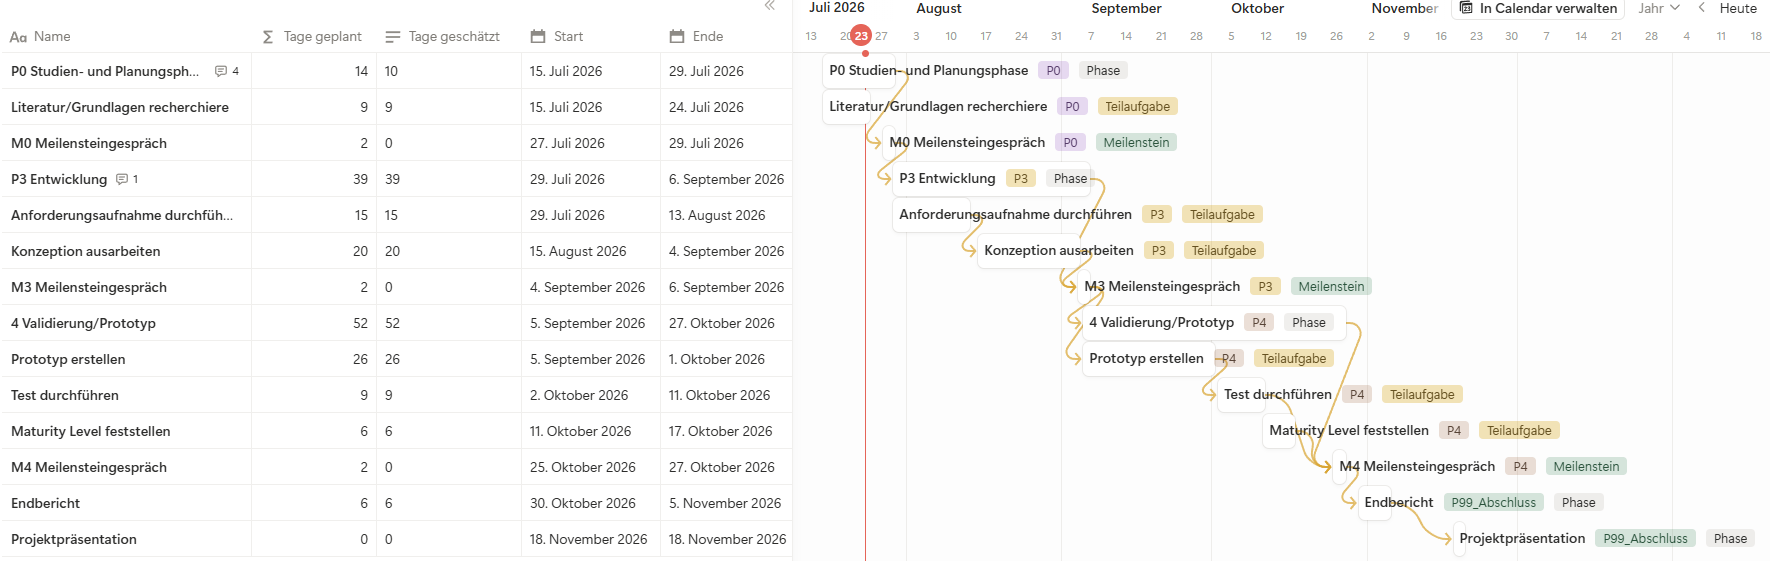
\includegraphics[width=\linewidth]{notion_proj_final.png}
    \captionof{figure}{Zeitplan}
    \label{fig:notiontimeline_full}
  \end{minipage}}
\vfill
\end{landscape}

\section{Stand der Forschung}

\subsection{Systematische Literatur Recherche}

Eine Systematische Literatur Recherche (SLR) wurde als methodologische Grundlage für die wissenschaftliche Betrachtung der für den Coasterbot nötigen Bestandteile durchgeführt.

Diese Fragen wurden für die SLR formuliert:

\begin{itemize}
  \item Welche Algorithmen zur Pfadfindung werden in mobilen IoT‑Geräten mit
    Abstandssensoren eingesetzt, um Kollisionen zu vermeiden?
  \item „Welche Algorithmen und Architekturen werden eingesetzt, um
    Inertialnavigation auf IoT‑Geräten mit begrenzten Ressourcen zu
    realisieren?“
  \item „Wie werden Inertialsensoren (IMU: Beschleunigungssensor, Gyroskop,
    ggf. Magnetometer) mit anderen Sensoren (z.B. GPS, Kamera, UWB) für robuste
    Navigation in IoT‑Systemen kombiniert?“
\end{itemize}

Diese Bestandteile der SLR wurden in die Kategorien „Mobile Roboter“ und
„Algorithmen“ eingeteilt.

Die Suche erfolgte neben IEEE Explore in frei zugänglichen Quellen (Google
Scholar, arXiv) aufgrund fehlender Zugänge zu lizenzierten Datenbanken wie
Scopus oder ACM Digital Library. Preprints aus arXiv wurden nur berücksichtigt,
wenn sie eine klar beschriebene Methodik und Evaluierung aufwiesen oder bereits
als Journal‑/Konferenzversion erschienen waren. Suchanfragen inklusive Link
befinden sich im Anhang.

\subsection{Recherche: Mobile Roboter}
Das Feld der mobilen Roboter ist bereits weit erforscht und es lassen sich eine Vielzahl an Arbeiten finden, die unterschiedliche Ansätze und Lösungen für die Navigation, Manipulation und Interaktion von Robotern in verschiedenen Umgebungen präsentieren. Eine übersichtliche Zusammenfassung relevanter Arbeiten ist in der Tabelle~\ref{tab:literaturrecherche-coasterbot} im Anhang dargestellt. Diese Tabelle enthält Informationen zu den jeweiligen Roboter-Projekten. Diese werden als Grundlage zur Bauteilauswahl und Softwarearchitektur des Coasterbots dienen. Insbesondere die Arbeit von~\cite{Balbuena2026Mar} kann als Grundlage dienen, da hier mehrere mobile Roboter Varianten vorgestellt und mit fertigen Stücklisten und CAD-Dateien veröffentlicht wurden. Damit bieten diese Arbeiten eine gute Grundlage für die Entwicklung des Coasterbots, so dass sich das Team auf die Softwarearchitektur, die Navigation des Roboters und die Hauptfunktion \textemdash~das Ablegen und Aufnehmen von Getränkeuntersetzer \textemdash~konzentrieren kann.


\subsection{Recherche: Algorithmen}


\subsubsection{Klassische Graphalgorithmen}

Die Grundlage vieler Verfahren zur autonomen Navigation bilden klassische
Graphalgorithmen. Dabei wird die Umgebung als Graph modelliert, dessen Knoten
diskrete Positionen oder Zustände repräsentieren, während Kanten mögliche
Bewegungen zwischen diesen beschreiben. Ziel ist die Bestimmung eines optimalen
Pfades hinsichtlich einer Kostenfunktion, beispielsweise der zurückgelegten
Distanz, Fahrzeit oder des Energieverbrauchs.

Ein Vertreter ist der Dijkstra-Algorithmus, der den kürzesten Pfad in Graphen
mit Kantengewichten berechnet. Der Algorithmus garantiert optimale Lösungen
insofern die Kantengewichte nicht-negativ sind und
stellt ein Referenzverfahren für die globale Pfadplanung in statischen
Umgebungen dar~\cite{Dijkstra}. Seine mathematische Grundlage sowie Laufzeitanalyse werden
ausführlich in „Introduction to Algorithms“ von Cornet et al.\ beschrieben~\cite{IntroToAlgs}.

Neben Dijkstra existieren weitere grundlegende Suchverfahren, wie die
Breitensuche (Breadth-First Search) und Tiefensuche (Depth-First Search,
DFS)~\cite{IntroToAlgs}.
Während BFS optimale Lösungen in ungewichteten Graphen liefert, dient DFS vor
allem der Strukturanalyse von Graphen und spielt in der Roboternavigation eine
untergeordnete Rolle.

Für Anwendungen mit einer vollständig bekannten und statischen Umgebung stellen
diese Algorithmen eine zuverlässige Grundlage der globalen Pfadplanung dar.

\subsubsection{Heuristische Verfahren}

Da klassische Graphalgorithmen bei großen Suchräumen einen hohen Rechenaufwand
verursachen, werden in der mobilen Robotik häufig heuristische Suchverfahren
eingesetzt. Ein bedeutendes Verfahren ist der heusristische A* Algorithmus, um
die Suche gezielt in Richtung des Zielknotens zu lenken~\cite{IntroToAlgs,AStar}.

Die Bewertung eines Knotens erfolgt über

\begin{equation}
f\left(n\right) = g\left(n\right) + h\left(n\right)
\end{equation}
%$$
%f(n) = g(n)+h(n)
%$$

Hierbei stellen $g(n)$ die wirklichen Kosten eines optimalen Pfades $s$ nach
$n$ und $h(n)$ die wirklichen Kosten eines optimalen Pfades von $n$ zu einem
präferierten Zielknoten von $n$ darstellt. Allgemein ist $h(n)$ eine Schätzung
der verbleibenden Distanz zum Ziel~\cite{AStar}. Ist die Heuristik zulässig (admissible),
garantiert A* ebenfalls optimale Lösungen, untersucht jedoch weniger Knoten als
Dijkstra.

Für mobile Roboter kommen häufig euklidische oder Manhattan-Distanzen~\cite{IntroToAlgs} als
Heuristik zum Einsatz. Dadurch eignet sich A* insbesondere für Gitternetze
(Occupancy Grids), wie sie in der Robotik genutzt werden\cite{RoboticMapping}.

Aktuellere Varianten wie Weighted A* oder Anytime A* priorisieren kürzere
Rechenzeiten gegenüber der optimalen Lösung, weshalb deren Anwendung geeignet in
Echtzeitsystemen ist\cite{WeightedA,AnytimeA}.

\subsubsection{Dynamische Pfadplanung}

In realen Einsatzgebieten verändert sich die Umgebung häufig während der Fahrt.
Statische Algorithmen müssten den gesamten Pfad erneut berechnen. Dies führt zu
hohen Rechenzeiten.

Hier setzen Verfahren der dynamischen Pfadplanung an. Zu nennen sind unter
anderem D* (Dynamic A*)~\cite{DAlg} sowie dessen Weiterentwicklung D* Lite~\cite{DLite}. Beide
Verfahren aktualisieren ausschließlich die von einer Umweltveränderung
betroffenen Bereiche des Suchgraphen und vermeiden dadurch vollständige
Neuberechnungen.

Ein weiteres relevantes Verfahren ist Lifelong Planning A* (LPA*), welches
inkrementelle Änderungen effizient verarbeitet~\cite{LifelongPlanningA}. Solche
Algorithmen werden insbesondere in autonomen Fahrzeugen und mobilen
Servicerobotern eingesetzt, deren Umgebungen durch Menschen oder bewegliche
Objekte beeinflusst werden.

Für einen Coaster Bot wären dynamische Planungsverfahren dann relevant, wenn
sich während der Navigation Gläser, Teller oder Personen im Arbeitsbereich
befinden.

\subsubsection{Kollisionsvermeidung}

Während globale Pfadplanung den optimalen Weg bestimmen, übernimmt die
Kollisionsvermeidung die kurzfristige Reaktion auf Hindernisse.

Ein Ansatz sind Potentialfeldmethoden, bei denen das Ziel eine anziehende Kraft
und Hindernisse abstoßende Kräfte erzeugen. Diese Methoden sind einfach
implementierbar, können jedoch in lokalen Minima stecken bleiben
~\cite{Potentialfeldmethoden}.

In mobilen Robotersystemen wird u.a.\ der Dynamic Window Approach (DWA)
verwendet, der die Bewegungsdynamik des Roboters selbst einbezieht
~\cite{DynamicWindowApproach}. Diese Strategie ist grundsätzlich ein statischer
Ansatz, der die Eigenschaften von Veränderungen in der Umgebung nicht
berücksichtigt. Durch den Einsatz von Neuronalen Netzen kann DWA, durch kurze
Observationen der sich verändernden Umgebung, die Bewegungen der Hindernisse
modellieren und somit auf Veränderungen der Umwelt reagieren
~\cite{DynamicAdaptiveDynamicWindowApproach}.

Für komplexe Konfigurationsräume kommen außerdem samplingbasierte Verfahren wie
Rapidly-exploring Random Trees (RRT)~\cite{RRT} sowie RRT*~\cite{RRTStar} zum Einsatz.
Während RRT schnell zulässige Pfade findet, verbessert RRT* diese schrittweise
bis zum asympotischen Optimum~\cite{RRTStar}.

Somit bildet die Kombination aus globalem Pfadplaner und lokaler
Kollisionsvermeidung einen möglichen Ansatz zur Bewegung des Coaster Bots dar.

\subsubsection{SLAM und Lokalisierung}

Zur verbesserten Navigation kann ein Roboter seine eigene Position bestimmen und
gleichzeitig eine Karte seiner Umgebung aufbauen. Dieses Problem wird als
Simultaneous Localization and Mapping (SLAM) bezeichnet~\cite{SLAM}.

Zu den klassischen Verfahren gehören Extended Kalman Filter (EKF-SLAM),
FastSLAM auf Basis von Paketfiltern sowie graphbasierte SLAM Verfahren~\cite{EKF,EKF-SLAM,FastSLAM}.

Besonders graphbasierte Optimierungsverfahren habe sich aufgrund ihrer hohen
Genauigkeit etabliert und bilden die Grundlage von Robotik-Frameworks wie ROS2
~\cite{ROS2}.

Für den Coaster Bot hängt die Bedeutung von SLAM vom Einsatzszenario und den
verwendeten Sensoren ab. Wird ausschließlich auf einem bekannten Tisch
gearbeitet, genügt meist eine vorher definierte Karte. Soll das System autonom
unbekannte Arbeitsbereiche erfassen oder sich frei im Raum bewegen können, ist
ein SLAM Verfahren vorteilhaft.

\subsubsection{Manipulationsplanung}

Neben der Navigation stellt die Manipulationsplanung einen wesentlichen
Bestandteil autonomer Serviceroboter dar. Sie umfasst die Planung und Steuerung
von Greifbewegungen sowie das sichere Aufnehmen und Ablegen von Objekten.
Hierbei müssen sowohl die Kinematik des Roboters als auch mögliche Kollisionen
zwischen Greifer, Objekt und Umgebung berücksichtigt werden
~\cite{ManipulationCBiRRT,MotionPlanning}.

Zur Bewegungsplanung von Roboterarmen werden häufig samplingbasierte Verfahren
wie RRT~\cite{RRT}, RRT*~\cite{RRTStar} oder Probabilistic Roadmaps (PRM)~\cite{PRM}
eingesetzt. Moderne Robotik-Frameworks wie MoveIt 2~\cite{MoveIt2} kombinieren diese
Planungsverfahren mit Kollisionsprüfungen und inverser Kinematik.

Für den Coaster Bot besteht die Manipulationsaufgabe darin, Getränkedeckel
präzise aufzunehmen und an einer definierten Zielposition abzulegen. Neben
einer genauen Positionierung des Roboters müssen dabei Greifstrategie,
Objektorientierung sowie eine zuverlässige Ablage berücksichtigt werden.

\subsubsection{Inertialnavigation}

Die Inertialnavigation (Inertial Navigation System, INS) beschreibt Verfahren
zur Bestimmung der Position, Orientierung und Bewegung eines mobilen Systems
ausschließlich auf Grundlage von Trägheitssensoren. Im Gegensatz zu
kamerabasierten oder laserbasierten Lokalisierungsmethoden ist die
Inertialnavigation nicht auf externe Referenzpunkte oder eine Sichtverbindung
zur Umgebung angewiesen. Dadurch eignet sie sich insbesondere für Anwendungen,
in denen optische Sensoren nur eingeschränkt eingesetzt werden können oder
zeitweise keine zuverlässigen Umgebungsinformationen zur Verfügung stehen
~\cite{IntegratedNavigationSystems,ModernRobotics}.

Ein Inertialnavigationssystem besteht zumeist aus einer Inertial
Measurement Unit (IMU), die Beschleunigungssensoren (Accelerometer) und
Drehratensensoren (Gyroskope) kombiniert. Moderne Systeme integrieren
zusätzlich Magnetometer zur Bestimmung der absoluten Orientierung. Aus den
gemessenen Beschleunigungen und Winkelgeschwindigkeiten werden durch numerische
Integration Geschwindigkeit, Orientierung und Position des Roboters berechnet.
Die mathematischen Grundlagen dieser Verfahren basieren auf den
Bewegungsgleichungen der klassischen Mechanik sowie auf Verfahren zur Schätzung
von Zustandsgrößen~\cite{IntegratedNavigationSystems,ModernRobotics}.

Ein Problem der Inertialnavigation stellt der Drift dar. Geringe Messfehler der
Sensoren werden durch die fortlaufende Integration akkumuliert und führen mit
zunehmender Betriebsdauer zu wachsenden Positions- und Orientierungsfehlern.
Aus diesem Grund wird eine reine Inertialnavigation in der mobilen Robotik nur
selten dauerhaft eingesetzt. Stattdessen erfolgt eine Kombination mit externen
Sensorsystemen wie LiDAR, Kameras oder Radencodern, um die Positionsschätzung
regelmäßig zu korrigieren~\cite{IntegratedNavigationSystems,ProbabilisticRobotics}.

Zur Fusion verschiedener Sensordaten kommen häufig probabilistische
Schätzverfahren wie der Kalman-Filter, der Extended Kalman Filter (EKF)~\cite{EKF}
oder der Unscented Kalman Filter (UKF)~\cite{UKF} zum Einsatz. Diese Verfahren
kombinieren die Messdaten der IMU mit absoluten Positionsinformationen anderer
Sensoren und ermöglichen dadurch eine robustere Lokalisierung. In aktuellen
Robotersystemen wird zudem vermehrt auf graphbasierte Optimierungsverfahren und
faktorgraphbasierte Ansätze zurückgegriffen, welche mehrere Sensordatenquellen
gleichzeitig berücksichtigen und die Genauigkeit der Positionsbestimmung
verbessern~\cite{ProbabilisticRobotics,HoB}.

Die Inertialnavigation findet in zahlreichen Bereichen der Robotik Anwendung.
Autonome Serviceroboter, fahrerlose Transportsysteme (AGV), Drohnen sowie
mobile Manipulatoren nutzen IMUs zur Stabilisierung der Bewegung, zur Schätzung
der Fahrzeuglage und zur kurzfristigen Positionsbestimmung. Besonders in
Innenräumen, in denen satellitengestützte Navigationssysteme wie GPS nicht
verfügbar sind, stellt die IMU eine wichtige Informationsquelle für die
Bewegungsregelung dar~\cite{GPS}. Auch in IoT- und Embedded-Systemen werden aufgrund der
geringen Baugröße, des niedrigen Energieverbrauchs und der geringen Kosten
häufig kompakte Micro-Electro-Mechanical Systems Inertial Measurement Units
(MEMS-IMUs) eingesetzt~\cite{ModernRobotics,HoB}.

Für den geplanten Coaster Bot kann die Inertialnavigation die globale
Pfadplanung und sensorbasierte Navigation ergänzen. Während Verfahren wie A*
oder Dijkstra den optimalen Fahrweg berechnen und LiDAR- oder
Kamerasysteme Hindernisse erkennen, liefert die IMU kontinuierlich
Informationen über Beschleunigung und Drehrichtung des
Roboters~\cite{AStar,IntroToAlgs}. Dadurch können
Fahrbewegungen zwischen Sensormessungen präziser geschätzt sowie kurzfristige
Positionsänderungen erfasst werden. Beim Anfahren definierter Ablage- oder
Aufnahmepositionen verbessert die Orientierungsschätzung die
Wiederholgenauigkeit des Systems. Die Kombination einer IMU mit Verfahren der
globalen Pfadplanung entspricht dem in der mobilen Robotik etablierten Ansatz
einer mehrstufigen Navigation~\cite{ModernRobotics,HoB}.

Da sich der Coaster Bot auf einer vergleichsweise kleinen Arbeitsfläche bewegt
und Bewegungen präzise erfolgen sollten,
ist eine alleinige Inertialnavigation aufgrund der Drift möglicherweise nicht
ausreichend. Eine mögliche Kombination aus mehreren Sensoren wie IMU,
Radencodern, einem LiDAR- oder kamerabasierten Lokalisierungssystem würden eine
effizientere Positionsbestimmung erreichen.


\newpage
\section{Anhänge}

\appendix

%acm bullshit
%\bibliographystyle{ACM-Reference-Format}
%\bibliography{quellen}

% normal scr article
\printbibliography[title={Literaturverzeichnis}]

\listoffigures


%\newpage
%\chapter*{References}
%\addcontentsline{toc}{chapter}{References}
%\printbibliography[heading=none]
\begin{landscape}
\section*{Literaturrecherche über mobile Roboter}
\begin{longtable}{@{} >{\raggedright\arraybackslash}p{3.0cm}
                      >{\raggedright\arraybackslash}p{2.6cm}
                      >{\raggedright\arraybackslash}p{3.4cm}
                      >{\raggedright\arraybackslash}p{5.0cm}
                      >{\raggedright\arraybackslash}p{5.4cm} @{}}
\caption{Vergleich mobiler Roboterplattformen aus der Literaturrecherche und Übertragbarkeit auf den Coasterbot}
\label{tab:literaturrecherche-coasterbot} \\
\toprule
\textbf{Roboter / Paper} & \textbf{Kategorie} & \textbf{Komponente} & \textbf{Details / Spezifikation} & \textbf{Übertragbarkeit auf Coasterbot} \\
\midrule
\endfirsthead

\multicolumn{5}{c}{{\tablename\ \thetable{} -- Fortsetzung von vorheriger Seite}} \\
\toprule
\textbf{Roboter / Paper} & \textbf{Kategorie} & \textbf{Komponente} & \textbf{Details / Spezifikation} & \textbf{Übertragbarkeit auf Coasterbot} \\
\midrule
\endhead

\midrule
\multicolumn{5}{r}{{Fortsetzung auf nächster Seite}} \\
\endfoot

\bottomrule
\endlastfoot

\multirow{11}{=}{Mona \cite{Arvin2019Jun}} & Mechanischer Aufbau & Leichtbau-Chassis & \textasciitilde{}45 g Gesamtgewicht, kompakte Bauform & Bedingt – Coasterbot braucht mehr Nutzlast (Untersetzer-Magazin, ggf. Getränke) \\
 & Mechanischer Aufbau & Räder \& Radstand & Raddurchmesser 28 mm, Radstand 80 mm & Als Referenzgröße für Mini-Prototyp geeignet \\
 & Aktor & 2x DC-Motor mit Untersetzungsgetriebe & Direktuntersetzung 250:1, symmetrischer Differentialantrieb & Hoch – Differentialantrieb ist Standardlösung für Coasterbot-Fahrwerk \\
 & Aktor & H-Brücken-Motortreiber & PWM-Ansteuerung je Motor, ca. 74 mW Leistungsbedarf & Hoch – Standard-Ansteuerung, direkt übertragbar \\
 & Sensor & 5x IR-Nahbereichssensor & 35° Sensorabstand, Hinderniserkennung/Bumper-Funktion & Mittel – für Personenerkennung ggf. zu kurze Reichweite, aber gut für Tischkantennähe \\
 & Sensor & Magnetischer Encoder & 6-Pol-Magnetscheibe + Hall-Sensor pro Motor, 1500 Pulse/Radumdrehung & Hoch – für Odometrie/Positionsregelung des Coasterbots relevant \\
 & Sensor & Spannungsteiler (Batterieüberwachung) & ADC-Messung der Akkuspannung & Hoch – einfache, günstige Lösung für Energiemanagement \\
 & Steuerung & ATmega328 Mikrocontroller & 8-bit AVR, 16 MHz, Arduino-kompatibel, 32 KB Flash & Hoch – ausreichend für Fahrsteuerung, ggf. zu schwach für Bilderkennung \\
 & Steuerung & Erweiterungsmodule (Raspberry Pi Zero, RF, WiFi, XBee) & Für höhere Rechenleistung/Kommunikation nachrüstbar & Hoch – Raspberry Pi als Rechen-Backbone für Vereinzelung/Erkennung denkbar \\
 & Software & Arduino IDE (C/C++) & Offene Programmierumgebung & Hoch – einfacher Einstieg für Prototyp-Firmware \\
 & Software & Stage-Simulator & 2D-Simulation von Multi-Robot-Szenarien & Gering – eher für Schwarmszenarien, für Einzelroboter-DoD nicht zwingend nötig \\
\midrule
\multirow{6}{=}{Diff.-Drive-Plattform \cite{Karakaya2022Apr}} & Mechanischer Aufbau & CAD-Chassis-Vollmodell & Solid-Modeling-Ansatz für Gesamtstruktur & Hoch – methodisches Vorbild für eigenes CAD/STL-Konzept \\
 & Mechanischer Aufbau & Antriebsrad-Befestigung & 3 Schrauben zwischen zwei gegenüberliegenden Scheiben, Bushings gegen Korrosion & Hoch – direkt anwendbares Konstruktionsdetail für Radanbindung \\
 & Aktor & DC-Motor (radachsnah montiert) & Motoren innenliegend entlang der Radachse & Hoch – platzsparende Motoranordnung fürs Chassis \\
 & Sensor & – (nicht spezifiziert) & Paper fokussiert rein mechanisch, keine Sensor-BOM & n/a \\
 & Steuerung & – (nicht spezifiziert) & Keine Angaben zu Controller/Elektronik & n/a \\
 & Software & CAD/Solid-Modeling-Software & Für mechanischen Entwurf verwendet & Hoch – Standardwerkzeug auch für STL-Erstellung im eigenen Projekt \\
\midrule
\multirow{5}{=}{Diff.-Drive Mobile Robot \cite{Hirpo2017Oct}} & Mechanischer Aufbau & 3D-Chassis-Modell & CAD-Baugruppe von Antriebs- und Castor-Rad & Mittel – gutes Referenzmodell, aber generisch \\
 & Aktor & 2x 12V-DC-Motor mit Getriebekopf & Bürsten-DC-Motor, Übersetzung n=3 & Hoch – Dimensionierungsbeispiel für Motorauswahl \\
 & Sensor & Tachometer/ Drehzahlgeber & Ktach = 1,8, zur Drehzahlrückführung & Hoch – für geschlossene Drehzahlregelung der Antriebsmotoren relevant \\
 & Steuerung & PID-Regler & Kp/Ki/Kd-Tuning für Drehzahlregelung & Hoch – Regelkonzept direkt für Fahrsteuerung übernehmbar \\
 & Software & MATLAB/Simulink & Modellierung \& Simulation des Regelkreises & Hoch – geeignet für die im DoD geforderte Ablaufsimulation \\
\midrule
\multirow{5}{=}{Edge Detecting Arduino Robot \cite{BibEntry2020Jul}} & Mechanischer Aufbau & Rad-Chassis (Kit-Basis) & Einfaches, kommerzielles Robot-Chassis & Gering – nur als didaktisches Beispiel, kein Custom-Design \\
 & Aktor & DC-Antriebsmotoren & Standard-Radantrieb & Gering – funktional redundant zu anderen Quellen \\
 & Sensor & IR-LED + IR-Fototransistor & Abwärts gerichtet, erkennt Tischkante/Cliff über fehlende Reflexion & Sehr hoch – Kernprinzip für die Tischkantenerkennung des Coasterbots \\
 & Steuerung & Arduino-Board & Einfacher Mikrocontroller zur Schwellenwert-Auswertung & Hoch – ausreichend für einfache Kantenerkennungslogik \\
 & Software & Arduino IDE, Schwellenwertlogik & Vergleich IR-Signal gegen festen Grenzwert & Hoch – einfachster Einstieg für Cliff-Detection-Funktion \\
\midrule
\multirow{6}{=}{Miniskybot \cite{Gonzalez-Gomez2012Jan}} & Mechanischer Aufbau & 3D-gedrucktes Chassis (9 Teile) & Front, Rear, 2 Räder, Batteriefach, -halter, 3-teiliges Castor-Rad & Sehr hoch – nahezu 1:1 übertragbares Konzept für STL-basierten Prototyp \\
 & Mechanischer Aufbau & O-Ring-Reifen \& M3-Verschraubung & Standard-O-Ringe als Bereifung, M3-Schrauben/Muttern & Hoch – kostengünstige, einfach zu beschaffende Lösung \\
 & Aktor & 2x modifizierter Hobby-Servomotor (Futaba 3003) & Für Dauerdrehung gehackt (Continuous Rotation) & Mittel – günstige Alternative zu DC-Motor+Getriebe, aber weniger präzise \\
 & Sensor & 2x SRF02-Ultraschallsensor & I2C-Bus, beliebig erweiterbar & Mittel – Ultraschall ggf. für Personen-/Hinderniserkennung nutzbar \\
 & Steuerung & PIC16F876A Mikrocontroller (Skycube-Board) & 8-bit, RS232-Programmierung, 4x AAA-Batterien & Mittel – funktional ausreichend, aber weniger verbreitet als Arduino/ATmega \\
 & Software & SDCC Cross-Compiler, OpenSCAD/FreeCAD, KiCad & Parametrisches CAD (Scripting) + offenes PCB-Design & Hoch – Open-Source-Toolchain für STL- und Schaltplan-Erstellung direkt nutzbar \\
\midrule
\multirow{10}{=}{Veter Robot \cite{BibEntry2018Dec}} & Mechanischer Aufbau & Dagu Rover 5 Kettenfahrwerk & Kommerzielles Tracked-Chassis als Basis & Gering – Kettenantrieb überdimensioniert für Coasterbot-Anwendung \\
 & Mechanischer Aufbau & 3D-gedruckter Aufbaukörper & Individuell anpassbarer Body für Sensorplatzierung & Hoch – Prinzip der modularen 3D-Druck-Karosserie übertragbar \\
 & Aktor & Sparkfun Dual-Motortreiber TB6612FNG & Ansteuerung der Rover-5-Antriebsmotoren & Hoch – bewährter, kompakter Motortreiber-IC \\
 & Aktor & Servomotor (rotierbarer Sensorkopf) & Für Ausrichtung von Kamera/Sonar & Mittel – evtl. für ausrichtbare Personendetektion nutzbar \\
 & Sensor & 3x Devantech SRF-02 + 1x SRF-08 Ultraschallsensor & Entfernungsmessung rund um den Roboter & Hoch – für Hindernis-/Tischkantenerkennung sowie Personenannäherung relevant \\
 & Sensor & Devantech CMPS10 Kompass & Digitaler Kompass/Neigungssensor & Gering – für Coasterbot-Anwendung (Innenraum, kurze Strecken) meist verzichtbar \\
 & Sensor & 2x Kamera + GPS-Empfänger & Für Bildverarbeitung und Außennavigation & Gering – GPS out of scope (Kartierung/Navigation), Kamera evtl. für Personenerkennung \\
 & Steuerung & BeagleBoard-xM (ARM+DSP) & Haupt-Recheneinheit für Bildverarbeitung/Kommunikation & Mittel – leistungsfähig, aber ggf. überdimensioniert; Raspberry Pi als Alternative \\
 & Steuerung & Pololu Power-Modul, Level-Shifter (Adafruit/Sparkfun) & Spannungswandlung \& Pegelanpassung zw. Logikebenen & Hoch – Standardkomponenten für saubere Spannungsversorgung \\
 & Software & On-/Offboard-Softwarestack (Git), Video-Streaming, OpenGL-Cockpit & Fernsteuerungs- und Telemetrie-Software & Gering – Fernsteuerung/Netzwerkanbindung ist laut DoD Out-of-Scope \\
\midrule
\multirow{9}{=}{e-puck \cite{BibEntry2026Jan}} & Mechanischer Aufbau & Zylindrisches Chassis & Ø 70 mm, Höhe 50 mm, Gewicht 200 g & Mittel – Formfaktor zu klein, aber Bauweise als Inspiration nutzbar \\
 & Aktor & 2x Schrittmotor mit Planetengetriebe & Präzise Positionierung, bis 13 cm/s & Mittel – Schrittmotoren bieten hohe Präzision, aber höhere Kosten als DC-Motor \\
 & Sensor & 8x IR-Näherungs-/Lichtsensor (TCRT1000) & Rundum-Hinderniserkennung + Umgebungslicht & Hoch – umlaufende Sensoranordnung als Vorbild für 360°-Erkennung \\
 & Sensor & \hspace{0pt}3D-Beschleunigungs\-sensor (IMU) & Lage-/Bewegungserkennung & Mittel – z. B. zur Erkennung von Kollisionen/Kippen nutzbar \\
 & Sensor & VGA-Farbkamera (640x480) & Für Bildverarbeitung/Objekterkennung & Hoch – für optionale Bestellaufnahme/Personenerkennung relevant \\
 & Sensor & 3x omnidirektionales Mikrofon & Richtungserkennung von Audioquellen & Gering – für Coasterbot-Kernfunktion nicht erforderlich \\
 & Steuerung & dsPIC-Mikrocontroller & 30–60 MHz, DSP-Kern, 8 KB RAM, 144 KB Flash & Mittel – leistungsfähig, aber proprietäres Ökosystem ggü. Arduino/ATmega \\
 & Steuerung & Bluetooth/RS232-Kommunikation & Kabellose Programmierung \& Fernsteuerung & Gering – Netzwerkanbindung laut DoD Out-of-Scope, ggf. nur für Debugging \\
 & Software & GNU GCC C-Compiler, Webots-Simulator & Offene Toolchain, 3D-Robotersimulation & Sehr hoch – Webots als möglicher Kandidat für die geforderte Programmablauf-Simulation \\
\midrule
\multirow{14}{=}{PlatROB \cite{Balbuena2026Mar}} & Mechanischer Aufbau & 4 modulare 3D-druckbare Baugruppen & Ackermann Drive Module (ADM), Omni-/Differential Drive Module (ODM/DDM), Control \& Processing Module (CPM), 4-DoF Manipulator (AMM) & Sehr hoch – modulares Baukastenprinzip direkt auf Fahr-/Spender-/Greifmodul des Coasterbots übertragbar \\
 & Mechanischer Aufbau & CPM-Chassis mit Wechselabdeckung & Trägt Jetson Nano \& Akkus, abnehmbarer Deckel für Kamera/LiDAR-Nachrüstung & Hoch – Konzept für wartungsfreundliches, erweiterbares Elektronikgehäuse \\
 & Aktor & Antriebsmotoren (Ackermann-Lenkung, Differential- \& Mecanum-Antrieb) & Austauschbare Fahrmodule je nach Anforderung (10 kg Nutzlast, 25 cm Wenderadius) & Hoch – Mecanum-/Differentialantrieb als Alternativkonzept für präzises Rangieren am Tisch \\
 & Aktor & 4-DoF Manipulator-Modul (AMM) & Roboterarm-Modul, 450 g Nutzlast, für Greif-/Manipulationsaufgaben & Sehr hoch – direkt relevant für Aufnahme/Abgabe von Untersetzern bzw. Flüssigkeitsaufnahme \\
 & Aktor & Motortreiber (auf Custom-PCB) & Ansteuerung der Antriebsmotoren je Fahrmodul & Hoch – Standardkomponente, gut dokumentiertes Referenzdesign \\
 & Sensor & 3x Ultraschallsensor (Hinderniserkennung) & Auf Custom-PCB des ODM/DDM integriert & Hoch – für Hindernis-/Personenerkennung rund um den Coasterbot nutzbar \\
 & Sensor & IMU (Inertial Measurement Unit) & Lageerkennung/Orientierung des Fahrmoduls & Mittel – z. B. zur Erkennung von Kippen oder unebenem Untergrund \\
 & Sensor & Motor-Encoder & Drehzahl-/Positionsrückführung je Antriebsmotor & Hoch – für Odometrie und präzises Anfahren am Tisch relevant \\
 & Sensor & Erweiterungs-Mounts (LiDAR, Kamera) & Vorgesehene Montagepunkte, nicht standardmäßig verbaut & Mittel – Kartierung ist laut DoD Out-of-Scope, Kamera für Personen-/Objekterkennung interessant \\
 & Steuerung & Arduino R3 Mikrocontroller (je Fahrmodul) & Steuert Motoren, Sensorik und I2C-Kommunikation je Modul & Hoch – bewährte, günstige Steuerungslösung für einzelne Subsysteme \\
 & Steuerung & NVIDIA Jetson Nano (CPM) & Zentrale Recheneinheit für KI-/Bildverarbeitungs-Workloads, 40–100 min Laufzeit & Hoch – geeignet als Hauptrechner für Personen-/Objekterkennung im optionalen Ausbau \\
 & Steuerung & Standardisierter I2C-Bus über DB9-Steckverbinder & Einheitliche Inter-Modul-Kommunikation zwischen allen Baugruppen & Sehr hoch – elegantes Konzept für saubere modulare Verkabelung (Fahr-/Spender-/Sensor-Modul) \\
 & Steuerung & 3x 18650 Li-Ion-Akku + Wippschalter/Relais & Energieversorgung inkl. einfacher Leistungsschaltung & Hoch – praxiserprobtes, günstiges Energiekonzept \\
 & Software & Teleoperations- \& Navigationssoftware, Open-Source-Repository (OSF) & Für Fernsteuerung und autonome Navigation genutzt; alle Baupläne/Firmware frei verfügbar & Hoch – guter Fundus für Software-Architektur-Referenz sowie Lizenzmodell (CC-BY 4.0) \\

\end{longtable}
\end{landscape}

\section*{Literaturrecherche der benötigte Algorithmen}
\subsection*{Pfadfindung und Kollisionsvermeidung}

IEEE Explore (Filter: 2014 bis 2026):
\begin{itemize}

\item \href{https://ieeexplore.ieee.org/search/searchresult.jsp?action=search&newsearch=true&matchBoolean=true&queryText=(\%22All\%20Metadata\%22:path\%20planning)\%20AND\%20(\%22All\%20Metadata\%22:collision\%20avoidance)\%20AND\%20(\%22All\%20Metadata\%22:mobile\%20robot)\&ranges=2014_2027_Year}
{("All Metadata":path planning) AND ("All Metadata":collision avoidance) AND ("All Metadata":mobile robot)}

\item \href{https://ieeexplore.ieee.org/search/searchresult.jsp?action=search&newsearch=true&matchBoolean=true&queryText=(\%22All\%20Metadata\%22:\%22path\%20planning\%22\%20AND\%20\%22All\%20Metadata\%22:\%22collision\%20avoidance\%22\%20AND\%20\%22All\%20Metadata\%22:\%22IoT\%22)\&ranges=2014_2027_Year}
{("All Metadata":"path planning" AND "All Metadata":"collision avoidance" AND "All Metadata":"IoT")}

\item \href{https://ieeexplore.ieee.org/search/searchresult.jsp?action=search&matchBoolean=true&newsearch=true&queryText=(TI:\%22path\%20planning\%22\%20AND\%20TI:\%22collision\%20avoidance\%22\%20AND\%20(TI:\%22mobile\%20robot\%22\%20OR\%20TI:\%22autonomous\%20robot\%22))}
{(TI:"path planning" AND TI:"collision avoidance" AND (TI:"mobile robot" OR TI:"autonomous robot"))}

\item \href{https://ieeexplore.ieee.org/search/searchresult.jsp?action=search&matchBoolean=true&queryText=((\%22ultrasonic\%20sensor\%22\%20OR\%20\%22ultrasonic\%20distance\%22)\%20AND\%20\%22mobile\%20robot\%22\%20AND\%20\%22navigation\%22)\&highlight=true\&returnFacets=ALL\&returnType=SEARCH\&matchPubs=true\&rowsPerPage=25\&ranges=2014_2026_Year}
{("ultrasonic sensor" OR "ultrasonic distance") AND "mobile robot" AND "navigation"}

\item \href{https://ieeexplore.ieee.org/search/searchresult.jsp?action=search&matchBoolean=true&queryText=((\%22optical\%20sensor\%22\%20OR\%20\%22light-dependent\%20resistor\%22)\%20AND\%20(\%22obstacle\%20detection\%22\%20OR\%20\%22edge\%20detection\%22)\%20AND\%20\%22navigation\%22)\&highlight=true\&returnFacets=ALL\&returnType=SEARCH\&matchPubs=true\&rowsPerPage=25\&ranges=2014_2025_Year}
{(("optical sensor" OR "light-dependent resistor") AND ("obstacle detection" OR "edge detection") AND "navigation")}

\item \href{https://ieeexplore.ieee.org/search/searchresult.jsp?action=search&matchBoolean=true&queryText=((\%22visual\%20SLAM\%22\%20OR\%20\%22monocular\%20SLAM\%22\%20OR\%20\%22stereo\%20vision\%22)\%20AND\%20(\%22collision\%20avoidance\%22\%20OR\%20\%22obstacle\%20detection\%22))\&highlight=true\&returnFacets=ALL\&returnType=SEARCH\&matchPubs=true\&rowsPerPage=25\&ranges=2014_2026_Year}
{("visual SLAM" OR "monocular SLAM" OR "stereo vision") AND ("collision avoidance" OR "obstacle detection")}

\item \href{https://ieeexplore.ieee.org/search/searchresult.jsp?action=search&matchBoolean=true&queryText=((\%22computer\%20vision\%22\%20AND\%20\%22path\%20planning\%22\%20AND\%20\%22mobile\%20robot\%22))\&highlight=true\&returnFacets=ALL\&returnType=SEARCH\&matchPubs=true\&rowsPerPage=25\&ranges=2014_2026_Year}
{("computer vision" AND "path planning" AND "mobile robot")}

\end{itemize}

\href{http://arXiv.org}{arXiv.org} (Filter: 2014--2026):
\begin{itemize}

    \item „Für arXiv wurden Boolesche Suchanfragen wie „inertial measurement unit” „sensor fusion” navigation „path planning” AND „obstacle avoidance” AND (“mobile robot” OR “autonomous robot”) sowie variationsreiche Kombinationen von Schlüsselwörtern zu Pfadfindung, Kollisionsvermeidung, Sensorik (Ultraschall, IR, Kamera, Lichtsensor) und IoT verwendet.“

    \item \href{https://arxiv.org/search/advanced?terms-0-operator=AND&terms-0-term=%22path+planning%22&terms-0-field=all&terms-1-operator=AND&terms-1-term=%22obstacle+avoidance%22&terms-1-field=title&terms-2-operator=AND&terms-2-term=%22mobile+robot%22&terms-2-field=title&terms-3-operator=OR&terms-3-term=autonomous+robot&terms-3-field=title&terms-4-operator=AND&terms-4-term=obstacle+avoidance&terms-4-field=title&classification-computer_science=y&classification-eess=y&classification-physics_archives=all&classification-include_cross_list=include&date-year=&date-filter_by=date_range&date-from_date=2014&date-to_date=2026&date-date_type=submitted_date&abstracts=show&size=50&order=-announced_date_first}
    {order: announced\_date\_first; size: 50; date\_range: 2014-01-01 to 2026-12-31; classification: Computer Science (cs), Electrical Engineering and Systems Science (eess); include\_cross\_list: True; terms: AND all="path planning"; AND title="obstacle avoidance"; AND title="mobile robot"; OR title="autonomous robot"; AND title="obstacle avoidance".}

    \item \href{https://arxiv.org/search/advanced?terms-0-operator=AND&terms-0-term=%22obstacle+avoidance%22+&terms-0-field=all&terms-1-operator=AND&terms-1-term=ultrasonic+sensor&terms-1-field=all&terms-2-operator=OR&terms-2-term=infrared+sensor&terms-2-field=title&terms-3-operator=AND&terms-3-term=distance+sensor&terms-3-field=title&classification-physics_archives=all&classification-include_cross_list=include&date-year=&date-filter_by=date_range&date-from_date=2014&date-to_date=2026&date-date_type=submitted_date&abstracts=show&size=50&order=-announced_date_first}
    {order: announced\_date\_first; size: 50; date\_range: 2014-01-01 to 2026-12-31; include\_cross\_list: True; terms: AND all="obstacle avoidance"; AND all="ultrasonic sensor"; OR title="infrared sensor"; AND title="distance sensor".}

    \item \href{https://arxiv.org/search/advanced?terms-0-operator=AND&terms-0-term=photoresistor+AND+robot&terms-0-field=all&terms-1-operator=OR&terms-1-term=+light+sensor&terms-1-field=title&terms-2-operator=OR&terms-2-term=light-dependent+resistor&terms-2-field=title&terms-3-operator=OR&terms-3-term=+line+following&terms-3-field=title&terms-4-operator=AND&terms-4-term=line+follower&terms-4-field=title&terms-5-operator=OR&terms-5-term=path+tracking&terms-5-field=title&classification-physics_archives=all&classification-include_cross_list=include&date-year=&date-filter_by=date_range&date-from_date=2014&date-to_date=2026&date-date_type=submitted_date&abstracts=show&size=50&order=-announced_date_first}
    {order: announced\_date\_first; size: 50; date\_range: 2014-01-01 to 2026-12-31; include\_cross\_list: True; terms: AND all="photoresistor" AND robot; OR title="light sensor"; OR title="light-dependent resistor"; OR title="line following"; AND title="line follower"; OR title="path tracking".}

\end{itemize}

Google Scholar (Filter: 2014--2026):
\begin{itemize}

    \item In Google Scholar wurden entsprechende Phrasensuchen wie
    path planning, collision avoidance, mobile robot bzw.
    vision-based, navigation, obstacle avoidance robot
    eingesetzt, der Veröffentlichungszeitraum wurde in der Regel auf 2014--2026 beschränkt.

    \item \href{https://scholar.google.com/scholar?q=%22path+planning%22+%22collision+avoidance%22+%22mobile+robot%22&hl=de&as_sdt=0%2C5&as_ylo=2014&as_yhi=2026}
    {\texttt{"path planning" "collision avoidance" "mobile robot"}}

    \item \href{https://scholar.google.com/scholar?hl=de&as_sdt=0%2C5&as_ylo=2014&as_yhi=2026&q=%22obstacle+avoidance%22+%22distance+sensor%22+%28IoT+OR+%22embedded+system%22%29&btnG=}
    {\texttt{"obstacle avoidance" "distance sensor" (IoT OR "embedded system")}}

    \item \href{https://scholar.google.com/scholar?hl=de&as_sdt=0%2C5&as_ylo=2014&as_yhi=2026&q=%22sensor-based+navigation%22+%22mobile+robot%22+obstacle&btnG=}
    {\texttt{"sensor-based navigation" "mobile robot" obstacle}}

    \item \href{https://scholar.google.com/scholar?hl=de&as_sdt=0%2C5&as_ylo=2014&as_yhi=2026&q=%22vision-based+navigation%22+%22obstacle+avoidance%22+robot&btnG=}
    {\texttt{"vision-based navigation" "obstacle avoidance" robot}}

    \item \href{https://scholar.google.com/scholar?hl=de&as_sdt=0%2C5&as_ylo=2014&as_yhi=2026&q=%28%22photoresistor%22+OR+%22light+sensor%22%29+%22line+following%22+robot&btnG=}
    {\texttt{("photoresistor" OR "light sensor") "line following" robot}}

    \item \href{https://scholar.google.com/scholar?hl=de&as_sdt=0%2C5&as_ylo=2014&as_yhi=2026&q=%22IoT+robot%22+%22path+planning%22+%22obstacle+avoidance%22&btnG=}
    {\texttt{"IoT robot" "path planning" "obstacle avoidance"}}

    \item \href{https://scholar.google.com/scholar?hl=de&as_sdt=0%2C5&as_ylo=2014&as_yhi=2026&q=%E2%80%9Cpath+planning%E2%80%9D+%E2%80%9Cobstacle+avoidance%E2%80%9D+%E2%80%9Cmobile+robot%E2%80%9D+%28IoT+OR+%E2%80%9Cwireless+sensor+network%E2%80%9D%29&btnG=}
    {\texttt{"path planning" "obstacle avoidance" "mobile robot" (IoT OR "wireless sensor network")}}

\end{itemize}

\subsection*{Inertialnavigation}

IEEE Explore (Filter: 2014--2026)
\begin{itemize}

   \item \href{https://ieeexplore.ieee.org/search/searchresult.jsp?action=search&newsearch=true&matchBoolean=true&queryText=(\%22All\%20Metadata\%22:\%22inertial\%20navigation\%22\%20)%20AND%20(%22All\%20Metadata\%22:IoT%20OR%20%22All\%20Metadata%22:%20%22Internet\%20of\%20Things%22%20%20OR%20%22embedded\%20system\%22%20OR%20%22microcontroller\%22)&ranges=2014_2026_Year}{("All Metadata":"inertial navigation") AND ("All Metadata":IoT OR "All Metadata":"Internet of Things" OR "embedded system" OR "microcontroller")}

    \item \href{https://ieeexplore.ieee.org/search/searchresult.jsp?action=search&newsearch=true&matchBoolean=true&queryText=(\%22inertial\%20navigation\%22\%20OR\%20\%22INS\%22)%20AND%20(\%22resource-constrained\%22\%20OR\%20\%22low-power\%22\%20OR\%20\%22low\%20power\%22\%20OR\%20\%22edge\%20device\%22)&ranges=2014_2026_Year}
    {("inertial navigation" OR "INS") AND ("resource-constrained" OR "low-power" OR "low power" OR "edge device")}

    \item \href{https://ieeexplore.ieee.org/search/searchresult.jsp?action=search&newsearch=true&matchBoolean=true&queryText=(\%22inertial\%20measurement\%20unit\%22\%20OR\%20IMU)%20AND%20navigation%20AND%20IoT&ranges=2014_2026_Year}
    {("inertial measurement unit" OR IMU) AND navigation AND IoT}

    \item \href{https://ieeexplore.ieee.org/search/searchresult.jsp?action=search&newsearch=true&matchBoolean=true&queryText=(\%22inertial\%20navigation\%22\%20OR\%20\%22inertial\%20odometry\%22)%20AND%20(\%22sensor\%20fusion\%22\%20OR\%20\%22Kalman\%20filter\%22\%20OR\%20\%22extended\%20Kalman\%22\%20OR\%20\%22particle\%20filter\%22)%20AND%20(IoT%20OR%20\%22embedded\%20system\%22)&ranges=2014_2026_Year}
    {("inertial navigation" OR "inertial odometry") AND ("sensor fusion" OR "Kalman filter" OR "extended Kalman" OR "particle filter") AND (IoT OR "embedded system")}

    \item \href{https://ieeexplore.ieee.org/search/searchresult.jsp?action=search&newsearch=true&matchBoolean=true&queryText=(\%22visual\%20inertial\%22\%20OR\%20\%22visual-inertial\%22)%20AND%20navigation%20AND%20(\%22mobile\%20robot\%22\%20OR%20drone%20OR%20UAV)&ranges=2014_2026_Year}
    {("visual inertial" OR "visual-inertial") AND navigation AND ("mobile robot" OR drone OR UAV)}

\end{itemize}


Google Scholar (Filter: 2014--2026)
\begin{itemize}

    \item \href{https://scholar.google.com/scholar?hl=de&as_sdt=0%2C5&as_ylo=2014&as_yhi=2026&q=%22inertial+navigation%22+%22IoT%22+%22resource-constrained%22+%22robot%22&btnG=}
    {\texttt{"inertial navigation" "IoT" "resource-constrained" "robot"}}

    \item \href{https://scholar.google.com/scholar?hl=de&as_sdt=0%2C5&as_ylo=2014&as_yhi=2026&q=%22inertial+navigation%22+%22embedded+system%22+%22microcontroller%22&btnG=}
    {\texttt{"inertial navigation" "embedded system" "microcontroller"}}

    \item \href{https://scholar.google.com/scholar?hl=de&as_sdt=0%2C5&as_ylo=2014&as_yhi=2026&q=%22AI-enhanced+inertial+navigation%22+IoT&btnG=}
    {\texttt{"AI-enhanced inertial navigation" IoT}}

    \item \href{https://scholar.google.com/scholar?hl=de&as_sdt=0%2C5&as_ylo=2014&as_yhi=2026&q=%22visual+inertial+navigation%22+%22mobile+robot%22&btnG=}
    {\texttt{"visual inertial navigation" "mobile robot"}}

    \item \href{https://scholar.google.com/scholar?hl=de&as_sdt=0%2C5&as_ylo=2014&as_yhi=2026&q=%22inertial+measurement+unit%22+%22sensor+fusion%22+navigation&btnG=}
    {\texttt{"inertial measurement unit" "sensor fusion" navigation}}

\end{itemize}

\end{document}
